\newpage
\chapter{Berechnung der Schnittkräfte}
\section{Berechnung der Lagerreaktionen der Hohlwelle}
\begin{center}
	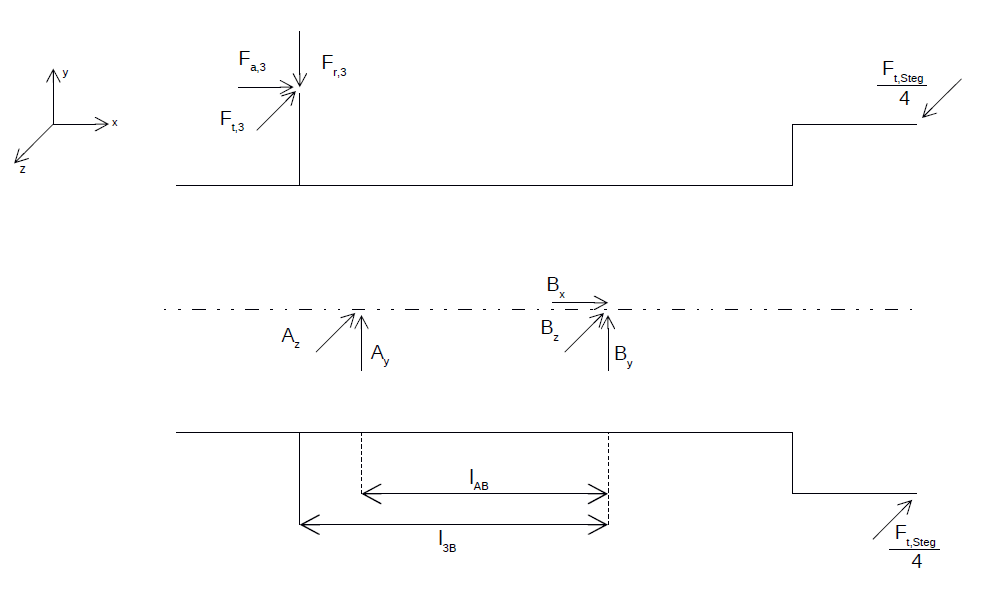
\includegraphics[width=1.04\textwidth,keepaspectratio]{figures/Hohlwelle.png}
\end{center}
\begin{itemize}
	\item Gegebene Werte: 
\begin{align*}
	&l_{AB} =171\text{ mm} \text{ , } l_{3B} = 175,8\text{ mm} \text{ , } d_{3} = 217,1\text{ mm}\\
	&F_{t,3} = 2633,53 \text{ N} \text{ , } F_{r,3}  = 1020,04\text{ N} \text{ , } F_{a,3} = 958,53 \text{ N}
\end{align*}
	\item Momentensummen:
\begin{align*}
	 \sum M\textsubscript{y}\textsuperscript{(B)} &\overset{!}{=} 0 = -A_z \x l_{AB} - F_{t,3} \x l_{3B} \\
	 	&\implies A_z = -F_{t,3} \x \frac{l_{3B}}{l_{AB}} = -2707,45 \text{ N} \\ \\
	 \sum M\textsubscript{z}\textsuperscript{(B)} &\overset{!}{=} 0 = -A_y \x l_{AB} + F_{r,3} \x l_{3B} - F_{a,3} \x \frac{d_3}{2}\\
	 	&\implies A_y = \frac{F_{r,3} \x l_{3B} - F_{a,3} \x \frac{d_3}{2}} {l_{AB}}= 440,2 \text{ N} 
\end{align*}
\end{itemize}
\section{Berechnung der Lagerreaktionen von Welle II}
\begin{center}
	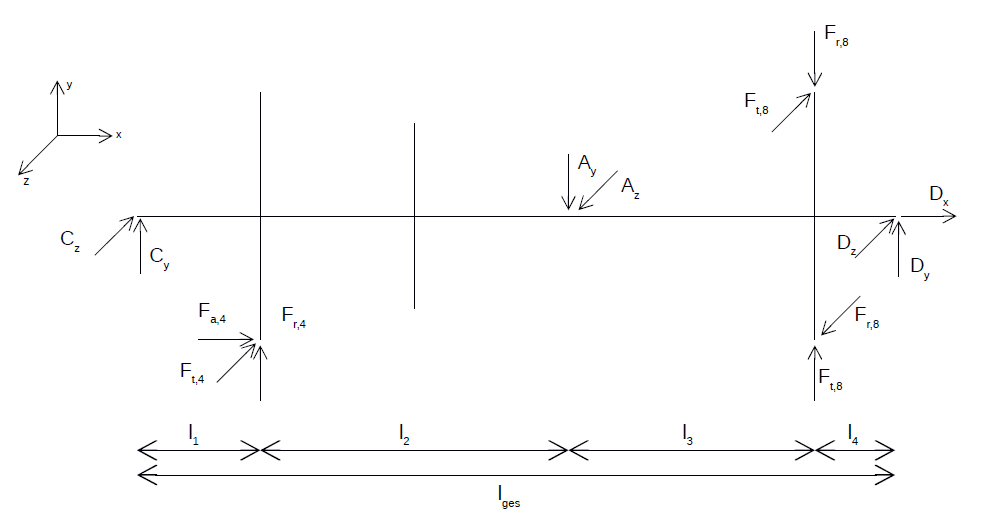
\includegraphics[width=1.04\textwidth,keepaspectratio]{figures/Uebersicht.png}
\end{center}
\begin{itemize}
	\item Gegebene Werte: 
	\begin{align*}
	&l_{1} =118,5\text{ mm} \text{ , } l_{2} = 226,5\text{ mm} \text{ , } l_{3} = 273 \text{ mm} \text{ , } l_{4} = 47\text{ mm} \text{ , } l_{ges} = 665\text{ mm} \\
	&d_4 = 89,4\text{ mm} \text{ , } d_8 = 112 \text{ mm} \\
	&F_{t,4} = 1598,88 \text{ N} \text{ , } F_{r,4}  = 619,29\text{ N} \text{ , } F_{a,4} = 581,94 \text{ N} \\
	&F_{t,8} = 319,1 \text{ N} \text{ , } F_{r,8}  = 116,13\text{ N}
\end{align*}
	\item Gleichgewichte:
\begin{align*}
    \sum F_x &\overset{!}{=} 0 = F_{a,4} + D_x \implies D_x = -F_{a,4} = -581,94 \text{ N} \\
    \sum F_y &\overset{!}{=} 0 = C_y + F_{r,4}-A_y +D_y - F_{r,8} + F_{r,8}\\ 
    \sum F_z &\overset{!}{=} 0 = A_z - C_z - D_z - F_{t,4} + F_{t,8} - F_{t,8}\\ \\
    \sum M\textsubscript{y}\textsuperscript{(D)} &\overset{!}{=} 0 = A_z \x (l_3+l_4)- F_{t,4} \x (l_2+l_3+l_4) - C_z \x l_{ges} +l_4 \x F_{t,8}- l_4 \x F_{t,8} \\ 
    &\implies C_z = \frac{(l_3+l_4) \x A_z - F_{t,4} \x (l_2+l_3+l_4)}{l_{ges}} = -2616,8 \text { N} \\ 
    & \implies D_z = A_z - C_z - F_{t,4}= -1689,53 \text{ N}\\ \\
    \sum M\textsubscript{z}\textsuperscript{(D)} &\overset{!}{=} 0 = (l_3+l_4) \x A_y + \frac{d_4}{2} \x F_{a,4} - (l_2+l_3+l_4) \x F_{r,4}- l_{ges} \x C_y  \\ 
    &\implies C_y = \frac{(l_3+l_4) \x A_y + \frac{d_4}{2} \x F_{a,4} - (l_2+l_3+l_4) \x F_{r,4}}{l\textsubscript{ges}} = -258 \text{ N}\\ 
    & \implies D_y =   A_y - C_y - F_{r,4} =  78,9\text{ N}\\ 
\end{align*}
\begin{align*}
    C_x &= \underline{0\text{ N}} & D_x= \underline{-581,94\text{ N}}\\
    C_y &= \underline{-258\text{ N}} & D_y= \underline{78,9\text{ N}}\\
    C_z &= \underline{-2616,8\text{ N}} & D_z= \underline{-1689,53\text{ N}}\\
\end{align*}
\end{itemize}
\newpage
\section{Berechnung der Schnittkraftverläufe}
\renewcommand{\labelenumi}{\roman{enumi})}
\begin{enumerate}
\item Bereich I: $0 \leq x_1 \leq l_1$
\begin{center}
	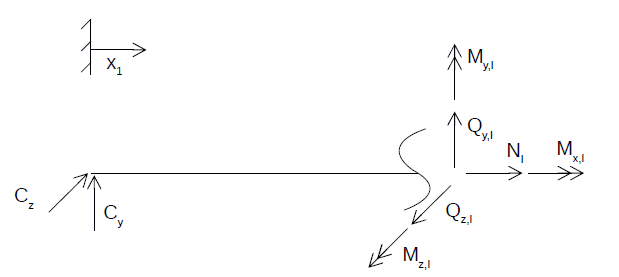
\includegraphics[width=1.04\textwidth,keepaspectratio]{figures/Bereich1.png}
\end{center}
    \begin{align*}
        \sum F_x &\overset{!}{=} 0 = N_{\mathrm{I}} \quad \implies \quad  N_{\mathrm{I}} = 0 \text{ N}\\ 
        \sum F_y &\overset{!}{=} 0 =  Q_{y,\mathrm{I}} + C_y \quad \implies \quad  Q_{y,\mathrm{I}} = -C_y = 258\text{ N}\\
        \sum F_z &\overset{!}{=} 0 =  Q_{z,\mathrm{I}} - C_z \quad \implies \quad  Q_{z,\mathrm{I}} = C_z = -2616,8\text{ N}\\
        \sum M_x \textsuperscript{(P)}&\overset{!}{=} 0 = M_{x,\mathrm{I}} \quad \implies \quad   M_{x,\mathrm{I}} = 0 \text{ Nm} \\ 
        \sum M_y \textsuperscript{(P)}&\overset{!}{=} 0 = M_{y,\mathrm{I}} - x_1 \x C_z \quad \implies \quad   M_{y,\mathrm{I}} =x_1 \x C_z =-2616,8 \text{ N} \x x_1\\ 
        \sum M_z \textsuperscript{(P)}&\overset{!}{=} 0 = M_{z,\mathrm{I}} -x_1 \x C_y  \quad \implies \quad   M_{z,\mathrm{I}} = x_1 \x C_y = -258 \text{ N} \x x_1 \\ 
    \end{align*}
\newpage
\item Bereich II: $0 \leq x_2 \leq l_2$
\begin{center}
	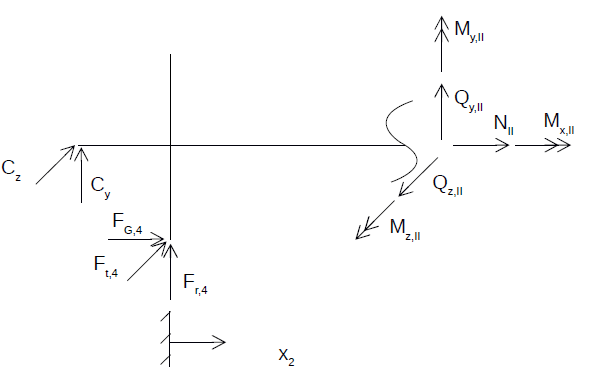
\includegraphics[width=0.93\textwidth,keepaspectratio]{figures/Bereich2.png}
\end{center}
\begin{align*}
        \sum F_x &\overset{!}{=} 0 = F_{a,4} + N_{\mathrm{II}} 
				\implies  N_{\mathrm{II}} = - F_{a,4}  =-581,94 \text{ N}\\ 
       \sum F_y &\overset{!}{=} 0 =C_y +F_{r,4} + Q_{y,\mathrm{II}} 
       		\implies  Q_{y,\mathrm{II}} = -C_y - F_{r,4} =-61,29 \text{ N}\\ 
       	\sum F_z &\overset{!}{=} 0 =-C_z -F_{t,4} + Q_{z,\mathrm{II}} 
       		\implies  Q_{z,\mathrm{II}} = C_z + F_{t,4} =-1017,92 \text{ N}\\ \\
        \sum M\textsubscript{x}\textsuperscript{(P)} &\overset{!}{=} 0 = M_{x,\mathrm{II}} + r_4 \x F_{t,4} \\
				&\implies M_{x,\mathrm{II}} = - \frac{d_4}{2} \x F_{t,4}  =  -71,5 \text{ Nm} \\ \\
		\sum M\textsubscript{y}\textsuperscript{(P)} &\overset{!}{=} 0 = M_{y,\mathrm{II}} - x_2 \x F_{t,4} - (l_1 + x_2) \x C_z \\
				&\implies M_{y,\mathrm{II}} = (l_1 + x_2) \x C_z +x_2 \x F_{t,4}  = -310,1\text{ Nm} -1017,92 \text{ N} \x x_2\\ \\
		\sum M\textsubscript{z}\textsuperscript{(P)} &\overset{!}{=} 0 = M_{z,\mathrm{II}} + \frac{d_4 }{2} \x F_{a,4} - x_2 \x F_{r,4} - (l_1 + x_2) \x )C_y \\ 
				&\implies M_{z,\mathrm{II}} = -\frac{d_4}{2} \x F_{a,4} + x_2 \x F_{r,4} + (l_1 + x_2) \x )C_y \\
				&= -56,59 \text{ Nm} + 361,29 \text{ N} \x x_2 \\
\end{align*}
\newpage
\item Bereich III: $0 \leq x_3 \leq l_3$
\begin{center}
	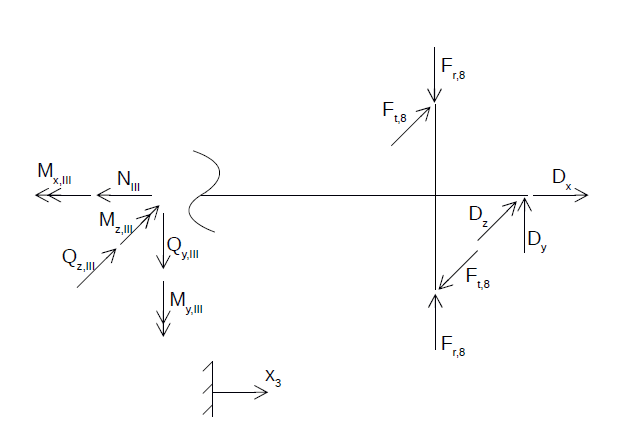
\includegraphics[width=0.93\textwidth,keepaspectratio]{figures/Bereich3.png}
\end{center}
	\begin{align*}
        \sum F_x &\overset{!}{=} 0 = D_x - N_{\mathrm{III}} 
				\implies  N_{\mathrm{III}} = D_x = -581,94 \text { N}\\ 
        \sum F_y &\overset{!}{=} 0 =D_y - Q_{y,\mathrm{III}} -F_{r,8} +F_{r,8}
				\implies Q_{y,\mathrm{III}} = D_y = 78,9 \text{ N}\\ 
		\sum F_z &\overset{!}{=} 0 = -D_z -Q{z,\mathrm{III}} +F_{t,8} - F_{t,8}
				\implies Q_{z,\mathrm{III}} = -D_z =1689,53 \text{ N} \\ \\
        \sum M\textsubscript{x}\textsuperscript{(P)} &\overset{!}{=} 0 =- M_{x,\mathrm{III}} - 4 \x \frac{d_8}{2}\x F_{t,8} \\
				&\implies M_{x,\mathrm{III}} = - 4 \x \frac{d_8}{2}\x F_{t,8} = -71,5 \text{ Nm} \\ \\
		\sum M\textsubscript{y}\textsuperscript{(P)} &\overset{!}{=} 0 =- M_{y,\mathrm{III}} + D_z \x (l_4+(l_3- x_3)) + F_{t,8} \x (l_3-x_3 )- F_{t,8} \x (l_3-x_3)\\
				&\implies M_{y,\mathrm{III}} = (l_4 + (l_3 - x_3)) \x D_z =-540,65 \text{ Nm} +1689,53 \text{ N} \x x_3\\ \\
		\sum M\textsubscript{z}\textsuperscript{(P)} &\overset{!}{=} 0 = - M_{z,\mathrm{III}} + D_y \x (l_4 + (l_3 - x_3)) + F_{r,8} \x (l_3 -x_3) - F_{r,8} \x (l_3 - x_3) \\
				&\implies  M_{z,\mathrm{III}} =  D_y \x (l_4 + (l_3 - x_3)) = 25,25 \text{ Nm} -78,9 \text{ N} \x x_3\\
	\end{align*}
\item Bereich IV: $0 \leq x_4 \leq l_4$
\begin{center}
	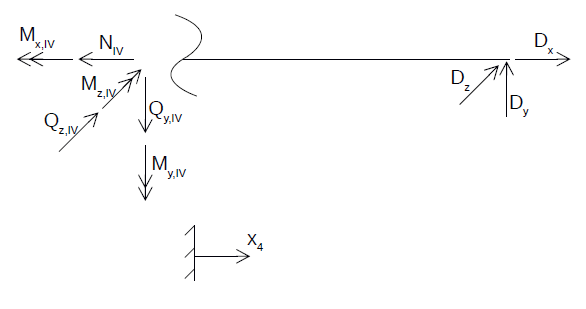
\includegraphics[width=1.04\textwidth,keepaspectratio]{figures/Bereich4.png}
\end{center}
\begin{align*}
	\sum F_x &\overset{!}{=} 0 = D_x - N_{\mathrm{IV}} 
		\implies  N_{\mathrm{IV}} = D_x = -581,94 \text { N}\\ 
	\sum F_y &\overset{!}{=} 0 =D_y - Q_{y,\mathrm{IV}}
		\implies Q_{y,\mathrm{IV}} = D_y = 78,9 \text{ N}\\ 
	\sum F_z &\overset{!}{=} 0 = -D_z -Q{z,\mathrm{IV}} 
		\implies Q_{z,\mathrm{IV}} = -D_z = 1689,53 \text{ N} \\ \\
	\sum M\textsubscript{x}\textsuperscript{(P)} &\overset{!}{=} 0 =- M_{x,\mathrm{IV}}  
		\implies M_{x,\mathrm{IV}} = 0 \text{ Nm} \\ \\
	\sum M\textsubscript{y}\textsuperscript{(P)} &\overset{!}{=} 0 =- M_{y,\mathrm{IV}} + D_z \x  (l_4 - x_4) \\
		&\implies M_{y,\mathrm{IV}} =  (l_4 - x_4) \x D_z =-79,4\text{ Nm} +1689,53 \text{ N} \x x_4\\ \\
	\sum M\textsubscript{z}\textsuperscript{(P)} &\overset{!}{=} 0 = - M_{z,\mathrm{IV}} + D_y \x  (l_4 - x_4)  \\
		&\implies  M_{z,\mathrm{IV}} =  D_y \x (l_4 - x_4) = 3,7\text{ Nm} -78,9 \text{ N} \x x_4
	\end{align*}
\end{enumerate}
\newpage
\textbf{Eckwerte:}\\ \\
Bereich i)
\begin{align*}
	N_{\mathrm{I}} (0) &= N_{\mathrm{I}} (l_1) = 0 \text{ N}\\
	Q_{y,\mathrm{I}} (0) &= Q_{y,\mathrm{I}} (l_1) = 258\text{ N}\\
	Q_{z,\mathrm{I}} (0) &= Q_{z,\mathrm{I}} (l_1) = -2616,8\text{ N}\\
	M_{x,\mathrm{I}} (0) &=  M_{x,\mathrm{I}} (l_1) = 0\text{ Nm}\\
	M_{y,\mathrm{I}} (0) &=  0\text{ Nm} & M_{y,\mathrm{I}} (l_1) &= -310,1\text{ Nm}\\
	M_{z,\mathrm{I}} (0) &= 0\text{ Nm} & M_{z,\mathrm{I}} (l_1) &= -30,57\text{ Nm}\\
\end{align*}
Bereich ii)
\begin{align*}
	N_{\mathrm{II}} (0) &= N_{\mathrm{II}} (l_2) = -581,94 \text{ N}\\
	Q_{y,\mathrm{II}} (0) &= Q_{y,\mathrm{II}} (l_2) =-61,29\text{ N}\\
	Q_{z,\mathrm{II}} (0) &= Q_{z,\mathrm{II}} (l_2) = -1017,92\text{ N}\\
	M_{x,\mathrm{II}} (0) &= M_{x,\mathrm{II}} (l_2) = -71,5\text{ Nm}\\
	M_{y,\mathrm{II}} (0) &=  -310,1 \text{ Nm} & M_{y,\mathrm{II}} (l_2) &= -540,65\text{ Nm}\\
	M_{z,\mathrm{II}} (0) &=  -56,59\text{ Nm} &M_{z,\mathrm{II}} (l_2) &= 25,25\text{ Nm}\\
\end{align*}
Bereich iii)
\begin{align*}
	N_{\mathrm{III}} (0) &= N_{\mathrm{III}} (l_3) = -581,94 \text{ N}\\
	Q_{y,\mathrm{III}} (0) &= Q_{y,\mathrm{III}} (l_3) =78,9\text{ N}\\
	Q_{z,\mathrm{III}} (0) &= Q_{z,\mathrm{III}} (l_3) = 1689,53\text{ N}\\
	M_{x,\mathrm{III}} (0) &= M_{x,\mathrm{III}} (l_3) = -71,5\text{ Nm}\\
	M_{y,\mathrm{III}} (0) &=  -540,65\text{ Nm} & M_{y,\mathrm{III}} (l_3) &= -79,4\text{ Nm}\\
	M_{z,\mathrm{III}} (0) &= 25,25\text{ Nm} &M_{z,\mathrm{III}} (l_3) &= 3,7\text{ Nm}\\
\end{align*}
Bereich iv)
\begin{align*}
	N_{\mathrm{IV}} (0) &= N_{\mathrm{IV}} (l_3) = -581,94 \text{ N}\\
	Q_{y,\mathrm{IV}} (0) &= Q_{y,\mathrm{IV}} (l_3) = 78,9\text{ N}\\
	Q_{z,\mathrm{IV}} (0) &= Q_{z,\mathrm{IV}} (l_3) = 1689,53\text{ N}\\
	M_{x,\mathrm{IV}} (0) &= M_{x,\mathrm{IV}} (l_3) = 0\text{ Nm}\\
	M_{y,\mathrm{IV}} (0) &=  -79,4\text{ Nm} & M_{y,\mathrm{IV}} (l_3) &= 0\text{ Nm}\\
	M_{z,\mathrm{IV}} (0) &= 3,7\text{ Nm} &M_{z,\mathrm{IV}} (l_3) &= 0\text{ Nm}\\
\end{align*}
\newpage
\section{Resultierende Momente}
\[
	|M_{b,res}(x)| = \sqrt{\left( M_{y}(x) \right)^2 + \left( M_{z}(x) \right)^2 }
\]
Bereich i)
\begin{align*}
	&|M_{b,res}(x=0)| = 0 \text{ Nm} \\
	&|M_{b,res}(x=l_1)| = 311,6 \text{ Nm} \\
\end{align*}
Bereich ii)
\begin{align*}
	&|M_{b,res}(x=l_1)| = 315,22 \text{ Nm} \\
	&|M_{b,res}(x=l_1+l_2)| = 541,24 \text{ Nm} \\
\end{align*}
Bereich iii)
\begin{align*}
	&|M_{b,res}(x=l_1+l_2)| = 541,24 \text{ Nm} \\
	&|M_{b,res}(x=l_1+l_2+l_3)| = 79,5 \text{ Nm} \\
\end{align*}
Bereich iv)
\begin{align*}
	&|M_{b,res}(x=l_1+l_2+l_3)| = 79,5 \text{ Nm} \\
	&|M_{b,res}(x=l_{ges})| = 0 \text{ Nm} \\
\end{align*}
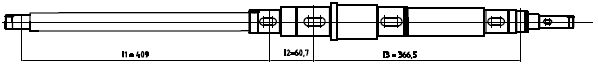
\includegraphics[width=\textwidth,keepaspectratio]{figures/Welle1klein.png}